\documentclass[12pt]{article}
\usepackage{amsmath}
\usepackage{array}
% \usepackage{gensymb}
\usepackage{geometry}
\usepackage{graphicx}
\usepackage{pgfplots}
\usepackage{siunitx}
\usepackage{wrapfig}

\title{Homework \#9}
\author{Donald Aingworth IV}
\date{October 16, 2024}

\pgfplotsset{width=8cm,compat=1.9}
\usepgfplotslibrary{external}
% \tikzexternalize

\begin{document}

\DeclareSIUnit{\mile}{mi}
\DeclareSIUnit{\gal}{gal}
\DeclareSIUnit{\foot}{ft}
\DeclareSIUnit{\h}{h}

% \maketitle

% \pagebreak
\section*{Problem 1}
A spring gun with k = 90.0 N/m is compressed by 5 cm. What is the exit speed of a 2.10-g projectile?

\subsection*{Solution}

\begin{align*}
    W   &= \int_{min}^{max} F(x)\ dx = \int_{-0.05}^{0} -kx\ dx = \left(-\frac{1}{2}kx^2\right)\vert_{-0.05}^{0} \\
        &= \frac{1}{2}k*0.05^2 = 45\unit{\newton/\meter} * 0.0025\unit{\meter^2} = 0.1 \unit{\joule}\\
    W   &=  \Delta K = K_f - K_i
\end{align*}
Since the spring on the block is unmoving at the start, then $v_i = 0$, so $K_i = \frac{1}{2}mv_i^2$ is also equal to zero. From there, we can determine the final kinetic energy and determine the velocity at the end.

\begin{align*}
    K_f &= W = 0.1\unit{\joule} = \frac{1}{2}mv_f^2\\
    \frac{2K_f}{m} &= v_f^2\\
    v_f &= \sqrt{\frac{2K_f}{m}} 
        = \sqrt{\frac{2*0.1\unit{\joule}}{0.0021\unit{\kilo\gram}}}
        = \sqrt{\frac{2*1000}{21}}\\
        &= \boxed{\frac{20\sqrt{105}}{21} \unit{\meter/\second} \approx 9.759 \unit{\meter/\second}}
\end{align*}

\pagebreak
\section*{Problem 2}
(a) The United States, with a population of $2.2 \times 10^8$ people, consumes $5 \times 10^{19}$ J per year. What is the per capita consumption in watts? (b) The sun's radiation provides the earth with 1000 \unit{\watt/\meter^2}. Assuming solar energy can be converted to electrical energy with a 20\% efficiency, how much area is needed to serve the energy needs of each U.S. citizen?

\subsection*{Solution}
\subsubsection*{Section (a)}
The power is determined by the work ($W$) divided by the time, with a watt being a joule divided by a second. The per capita value is determined by division by the number of humans ($c$). Assuming a year of 365 days, we can calculate the number of seconds per year ($t$) first.
\begin{align*}
    t   &=  1 \text{ years} * \frac{365\text{ days}}{1\text{ years}} 
                            * \frac{24\text{ hours}}{1\text{ days}}
                            * \frac{3600\unit{\second}}{1\text{ hours}}
        =   31536 \times 10^3 \unit{\second}\\
    P   &=  \frac{W}{t}
        =   \frac{5 \times 10^{19} \unit{\joule}}{(31536 \times 10^3 \unit{\second})}
        =   \frac{5 \times 10^{16}}{31536} \unit{\watt}\\
        &=  1.58549 \times 10^{12}\ \unit{\watt}\\
    P_{per\ captia}  &=  \frac{1.58549 \times 10^{12}}{2.2 \times 10^8} \unit{\watt}\\
        &=  \boxed{ 7206.77 \unit{\watt} }
\end{align*}

\subsubsection*{Section (b)}
Since there is only a 20\% efficiency, the usable numbers of watts per square meter would be $ Wa = 1000\ \unit{\watt/\meter^2}*\frac{20}{100} = 200\ \unit{\watt/\meter^2} $. We can divide the total power necessary per citizen (which we calculated in part (a)) to get the area necessary.
\begin{align*}
    A   &= \frac{P}{Wa}
        = \frac{ 7206.77 \unit{\watt} }{ 200\ \unit{\watt/\meter^2} }
        = \boxed{36.03 \unit{\meter^2}}
\end{align*}

\pagebreak
\section*{Problem 3}
A 0.595-kg object is released from a height of 3.60 m and lands on the ground. Find: (a) the work done by gravity; (b) the change in kinetic energy of the ball; (c) the speed just before it lands using energy methods. Ignore air resistance.

\subsection*{Solution}
\subsubsection*{Section (a)}
The object is released directly downward, so the angle with the vertical would be $ \phi = 90 \unit{\degree} = \frac{\pi}{2} $, so $\cos(\phi) = \cos(\frac{\pi}{2}) = 1$. This simplifies the formula from $W_g = mgd\cos(\phi)$ to $W_g = mgd$.
\begin{align*}
    W_g &=  mgd
        =   0.595\unit{\kilo\gram} * 9.81\unit{\meter/\second^2} * 3.60 \unit{\meter} 
        =   \boxed{21.01302\unit{\joule}}
\end{align*}

\subsubsection*{Section (b)}
The change in kinetic energy is equal to the work done by it. Since the object is in freefall, the only work done on it is the gravitational work.
\[ \Delta K = W_g = \boxed{21.01302\unit{\joule}} \]

\subsubsection*{Section (c)}
We can here use the formula for kinetic energy given the change in kinetic energy. The initial kinetic energy, since it starts from no velocity, is zero.
\[ \Delta K = K_f - K_i = K_f - 0 = K_f \]
\begin{align*}
    \Delta K    = K_f   &= \frac{1}{2}mv_f^2\\
    v_f^2   &=  \frac{2K_f}{m} = \frac{2*21.01302\unit{\joule}}{0.595\unit{\kilo\gram}} = 70.632 \unit{\meter^2/\second^2}\\
    v_f     &=  \sqrt{70.632 \unit{\meter^2/\second^2}} = \boxed{8.4043 \unit{\meter/\second}}
\end{align*}

\pagebreak
\section*{Problem 4}
\begin{wrapfigure}{r}{0.35\textwidth}
    \vspace{-30pt}
    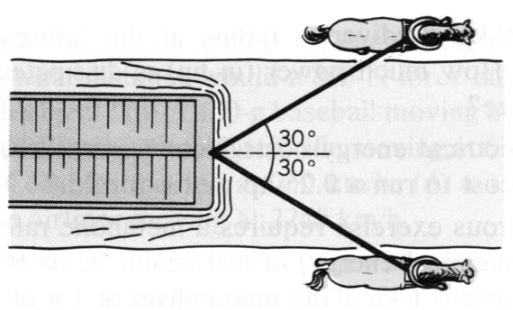
\includegraphics[width=0.35\textwidth]{graph_4.png} 
    % \label{fig:wrapfig}
\end{wrapfigure}
Two horses pull a barge along a canal at a steady 5.00 km/h, as shown in the figure. The tension in each rope is 420 N and each is at 30\unit{\degree} to the direction of motion. What is the horsepower provided by the horses?

\subsection*{Solution}
First, we convert units from km/h to m/s. 
\[ 5.00 \unit{\kilo\meter/\hour} * \frac{1000 \unit{\hour*\meter}}{3600 \unit{\kilo\meter*\second}} = \frac{25}{18} \unit{\meter/\second} \]

Now, we calculate from the tension the horizontal force exerted by each horse.
\[ F_x = T\cos(\phi) = 420\unit{\newton} * \cos(30\unit{\degree}) = 210*\sqrt{3}\unit{\newton} \]

Next, we multiply this force by the velocity of the horses to find the power of each individual horse, then multiply that by two to find the total horse power.
\begin{eqnarray*}
    P = F_x*v = (210*\sqrt{3}\unit{\newton}) * (\frac{25}{18} \unit{\meter/\second}) = \frac{875\sqrt{3}}{3} \unit{\watt}\\
    2*P = 2*\frac{875\sqrt{3}}{3} \unit{\watt} = \frac{1750\sqrt{3}}{3} \unit{\watt} = \boxed{1010.36 \unit{\watt}}
\end{eqnarray*}

\pagebreak
\section*{Problem 5}
\begin{wrapfigure}{r}{0.35\textwidth}
    \vspace{-30pt}
    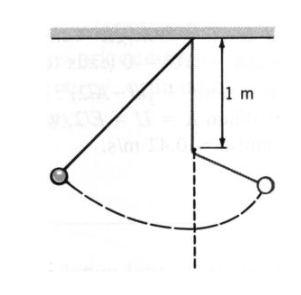
\includegraphics[width=0.35\textwidth]{graph_5.png} 
    % \label{fig:wrapfig}
\end{wrapfigure}
A pendulum bob of mass 0.710 kg is suspended by a string of length 1.50 m. The bob is released from rest
when the string is at 30\unit{\degree} to the vertical. The swing is interrupted by a peg 1.00 m vertically below the support
as shown below. What is the maximum angle to the vertical made by the string after it hits the peg?

\subsection*{Solution}
In this instance, the work done by gravity on the way down would have to be equal to the work loston the way up. The distance that the bob would fall down would be equal to the maximum distance down minus the length of the string the cosine of the angle the string makes with the vertical. The same applies for the distance the bob would go back up after the interruption.
\begin{align*}
    W_{down} &= W_{up}\\
    mgh_1 &= mgh_2\\
    h_1 &= h_2\\
    L_1 - L_1\cos(\theta) &= L_2 - L_2\cos(\phi)\\
    \frac{L_1}{L_2}(1-\cos(\theta)) &= 1 - \cos(\phi)\\
    \cos(\phi) &= 1 - \frac{L_1\cos(\theta)}{L_2}\\
    \phi &= \arccos\left(1 - \frac{1.5\unit{\meter}*(1 - \cos(30\unit{\degree}))}{0.5\unit{\meter}}\right)\\
    \phi    &=  \boxed{53.26\unit{\degree}}
\end{align*}

\pagebreak
\section*{Problem 6}
\begin{wrapfigure}{r}{0.35\textwidth}
    \vspace{-30pt}
    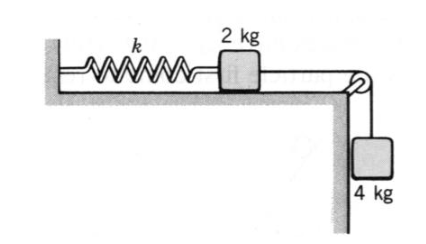
\includegraphics[width=0.35\textwidth]{graph_6.png} 
    % \label{fig:wrapfig}
\end{wrapfigure}
A 2.00-kg block slides on a frictionless horizontal surface and is connected on one side to a spring with a spring constant of 45.0 N/m, as shown the figure. The other side is connected to a 4.00-kg block that hangs vertically. The system starts from rest with the spring unextended. (a) What is the maximum extension of the spring? (b) What is the speed of the 4.00-kg block when the extension is 50 cm?

\subsection*{Solution}
\subsubsection*{Section (a)}
Assuming the direction away from the wall to be positive, we do this. The mass here used will be the mass of the 4.00-kg block. 
\begin{align*}
    F_s &= -kx\\
    F_{net\ 2} = 0 &= mg - T\\
    F_{net\ 1} = 0 &= T - kx\\
    0   &=  mg - kx\\
    kx  &=  mg\\
    x   &=  \frac{mg}{k} = \frac{4\unit{\kilo\gram}*9.81\unit{\meter/\second^2}}{45\unit{\newton/\meter}} = \boxed{0.872\unit{\meter}}
\end{align*}

\subsubsection*{Section (b)}
We here use the formula for the spring work at 50-cm and then use that to calculate the kinetic energy and velocity at that point. We also use the total mass of the two blocks together, which is 2.00-kg + 4.00-kg = 6.00-kg.
\begin{align*}
    W_s &=  \frac{1}{2} kx^2 = \frac{45*(0.5\unit{\meter})^2}{2} = \frac{45}{8}\\
    K   &=  \frac{1}{2}mv^2 = 3\unit{\kilo\gram}*v^2 = \frac{45}{8}\\
    v^2 &=  \frac{15}{8}\rightarrow
    v   &=  \sqrt{\frac{15}{8}} = \boxed{\frac{3*\sqrt{10}}{4} \unit{\meter/\second} = 2.37 \unit{\meter/\second}}
\end{align*}

\pagebreak
\section*{Problem 7}
\begin{wrapfigure}{r}{0.35\textwidth}
    \vspace{-30pt}
    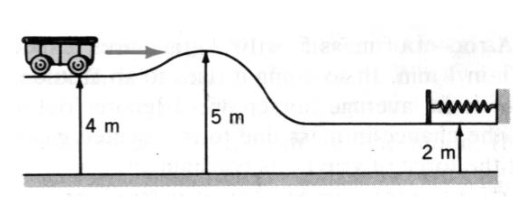
\includegraphics[width=0.35\textwidth]{graph_7.png} 
    % \label{fig:wrapfig}
\end{wrapfigure}
A cart with a mass of 3.20 kg, an initial speed of 5.15 m/s and an initial height of 4.00 m is moving towards a hill of height 5.00 m, as shown in the figure. On the other side of the hill is a spring with a spring constant of 125 N/m and a height of 2.00 m. (a) Does the trolley reach the spring? (b) If so, what is the maximum compression? Ignore frictional losses and the rotational energy of the wheels.

\subsection*{Solution}
\subsubsection*{Section (a)}
For the trolley to make it up the hill, the gravitational work would have to be less than the starting kinetic energy. Ths means that this must be the case: 
\begin{align*}
    K &> W_g \\ 
    \frac{1}{2}mv^2 &> mgh \\ 
    (5.15\unit{\meter/\second})^2 &> 2*9.81\unit{\meter/\second^2}*1\unit{\meter} \\
    26.5225\unit{\meter^2/\second^2} &> 19.72\unit{\meter^2/\second^2}
\end{align*}
Since it's all downhill from the top of the hill, the trolley \textbf{does reach the spring}.

\subsubsection*{Section (b)}
First we find the kinetic energy after it lowers by a net total of 2-m. 
\begin{align*}
    \Delta K = W_g &= K_f - K_i\\
    K_f &=  K_i + W_g
        =   \frac{1}{2}mv_i^2 + mg(\Delta h)\\
        &=  3.20\unit{\kilo\gram}(26.5225 + 9.81*2.00)\unit{\meter^2/\second^2} = 147.656\unit{\joule}
\end{align*}

For us to find the compression of the spring, we would know that the work done by the spring would be equal to the kinetic energy going in.
\begin{align*}
    W_s = \frac{1}{2}kx^2 &= 147.656\unit{\joule} = K_f\\
    x^2 &= \frac{295.312\unit{\joule}}{125\unit{\newton/\meter}} = 2.362\unit{\meter^2} \Rightarrow x = \boxed{1.537\unit{\meter}}
\end{align*}

% \pagebreak
% \section*{Problem 8}


% \subsection*{Solution}


\end{document}